\PassOptionsToPackage{quiet}{fontspec} 
\documentclass{ctexart}
\usepackage{lipsum}
\usepackage{xcolor,listings}
\usepackage{graphicx,float}
\graphicspath{{imgs/}}
% \ctexset{section={format+=\raggedright}}
\lstset{
    showstringspaces=false,
    frame=single,
    numbers=left,
    numberstyle=\color{darkgray},
    backgroundcolor=\color{white},
    keywordstyle=\color{blue},
    commentstyle=\it\color[RGB]{0,100,0},
    stringstyle=\sl\color{red},
}
\begin{document}
\title{数字图像处理基础-图书ISBN号字符识别}
\author{覃梓鑫(软工2003-20202005175)}
\date{\today}
\maketitle
\tableofcontents
\newpage
\section{概述}
\noindent
\textbf{设计目的:}\\
\textbf{内容:}\\
\textbf{运行环境:}
Windows10 + Python 3.10.6\\
所需 Python 第三方库如下:
\begin{itemize}
    \item 略
\end{itemize}
\noindent
\textbf{开发工具:}%不用加多余的\\
\begin{itemize}
    \item 操作系统 Windows 10 21H2
    \item 集成开发环境 Visual Studio Code 1.73.1
    \item 文档编写工具 TeXworks 0.6.6
    \item 编程语言 Python 3.10.6
          % \item 版本管理工具 git 2.29.0
    \item 编码格式 UTF8
\end{itemize}

\section{整体设计}
\section{具体实现}
\textit{为了表述的方便,该节按照模块进行分节,并在每个模块内部分别描述其具体必要的程序框图、数学模型、核心程序与处理过程图片。}
\subsection{灰度化}
根据课件(第11章-P38页-4彩色平衡)内容可知,彩色图像数字化后,景物颜色会偏移真实颜色,导致三基色不平衡。这里采用白平衡法计算灰度,即使用公式:%不需要\\
\[I(x,y)=0.299\cdot f_R(x,y)+0.587\cdot f_G(x,y)+0.114\cdot f_B(x,y)\] %不需要\\
但是如果直接使用Python迭代来处理上述过程,非常缓慢。所以考虑用\textbf{矩阵运算优化}。我们知道,向量内积的计算结果是实数,故有:
\[(R,G,B)\cdot(0.299,0.587,0.114)=0.299R+0.587G+0.114B\]
因此,考虑用向量内积,直接调用底层依托 C++ 实现的 numpy 的向量运算 dot 函数,一来 C++ 比 Python 快,二来矩阵运算比迭代快,这样能起到不小的常数优化作用。在下文的其他具体实现里也会反复用到类似的思路。因此,核心代码如下:
\begin{lstlisting}[language=python]
import numpy as np
def toGrey(img):
    if len(img.shape) == 2:  # 已经是灰度图像了
        return img
    rd = img.shape[2]  # 可能是3/4(png有alpha通道)
    line = [0.299, 0.587, 0.114, 0][:rd]
    trans = np.array(line).transpose()  # 矩阵转置
    img2 = np.dot(img, trans).astype(img.dtype)
    img2 = np.reshape(img2, img.shape[:2])
    return img2
\end{lstlisting}
运行效果如下:
\begin{figure}[htbp]
    \centering
    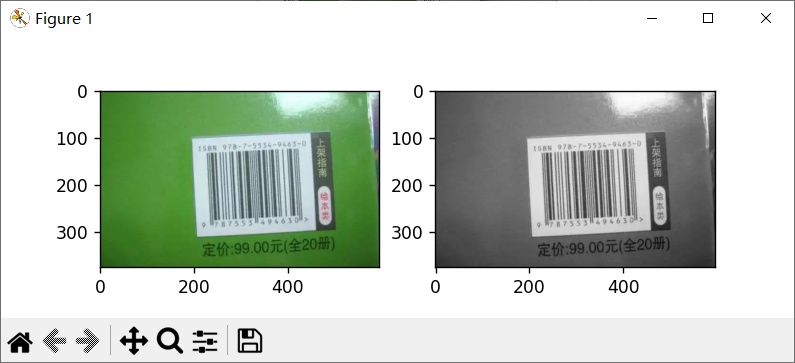
\includegraphics[height=120pt]{sample_toGrey}
    \caption{灰度化效果展示}
\end{figure}


\subsection{二值化}
根据课件(第9章-3基于阈值的图像分割)内容可知,可以按照图像的灰度不同,选取一个阈值 $x$,将灰度 $\ge x$ 的都转为一种灰度,其余的转为另一种灰度,实现二值化。这个阈值如果手动选取的话适应性不够强,所以考虑用基本自适应阈值。采用 Otsu 算法(最大类间方差法),具体步骤如下:
设图像长宽为 $n,m$,最佳阈值是 $x$,$< x$ 的点有 $n_0$ 个,$\ge x$ 的点有 $n_1$ 个,原图 $< x$ 的点平均灰度为 $\mu_0$,$\ge x$ 的点平均灰度为 $\mu_1$,令:
\[w_0=\frac{n_0}{nm},\quad w_1=\frac{n_1}{nm}\]
显然满足:
\[n_0+n_1=nm,\quad w_0+w_1=1\]
则二值化前的均值 $\mu$ 显然满足:
\[\mu=w_0\cdot\mu_0+w_1\cdot\mu_1\]
为了让方差最大化,设方差 $\sigma$ 为:
\[\sigma=w_0\cdot(\mu_0-\mu)^2+w_1\cdot(\mu_1-\mu)^2\]

联立解得:$\sigma=w_0\cdot w_1\cdot (\mu_0-\mu_1)^2$,因此,将所有 $\ge x$ 的点与 $< x$ 的点分别染色为两种灰度,即可实现灰度化。

具体到代码实现上,可以枚举 $x\in[0,255]$,然后分别计算 $\sigma$,将取得最大 $\sigma$ 的 $x$ 作为阈值即可。

考虑到在本题中,一般是从按的背景上分割出暗的物体(即数字),所以将 $< x$ 的都染为黑色,$\ge x$ 的都染成白色。

上述代码涉及大量遍历图像的操作,将其用\textbf{矩阵运算优化},能显著提升运算效率。时间复杂度为 $O(255nm)$,对较小的图像能以几乎一瞬间求出结果。

核心代码如下:
\begin{lstlisting}[language=python]
import numpy as np
def getThrestHold(img):
    n, m = img.shape
    mx, x = -1, 0  # mx是当前最大值,x是取得最值的阈值
    np.seterr(divide='ignore',invalid='ignore')#零除
    for i in range(0, 256):
        n0 = np.sum(img < i)
        n1 = n*m-n0
        w0 = n0/(n*m)
        w1 = 1-w0
        mu0 = np.sum(img[img < i])/n0
        mu1 = np.sum(img[img >= i])/n1
        g = w0*w1*(mu0-mu1)**2
        if g > mx:
            mx, x = g, i
    return x
def toBinary(img, x, ltx=0, gex=255):
    img2 = img.copy()
    img2[img2 < x] = ltx
    img2[img2 >= x] = gex
    return img2
\end{lstlisting}
运行效果如下:
\begin{figure}[htbp]
    \centering
    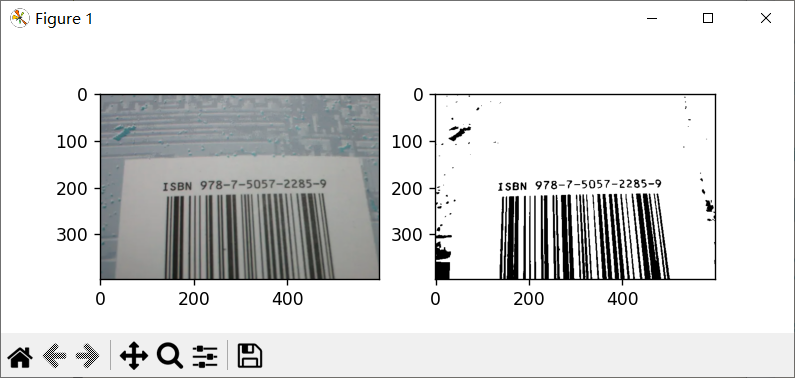
\includegraphics[height=120pt]{sample_toBinary}
    \caption{二值化效果展示}
\end{figure}


\subsection{字符定位及分割}
基本原理:将图片二值化之后(假设背景是白色,其余是黑色),在理想情况下(没有旋转、没有多余内容、噪声等),如果统计每一行每一列有多少个黑点,绘制水平和垂直统计图。核心代码如下:
\begin{lstlisting}[language=python]
def getHoriAndVertSum(img):
    img1 = ((255-img)//255).astype(np.uint16)
    sumVert = img1.sum(axis=0)
    sumHori = img1.sum(axis=1)
    return [sumHori, sumVert]
\end{lstlisting}
可以发现ISBN的部分会呈现出一段特殊波的形状,如图所示:\textit{(作图代码见附录)}
\begin{figure}[H]%让插入的图片紧跟在文字后面
    \centering
    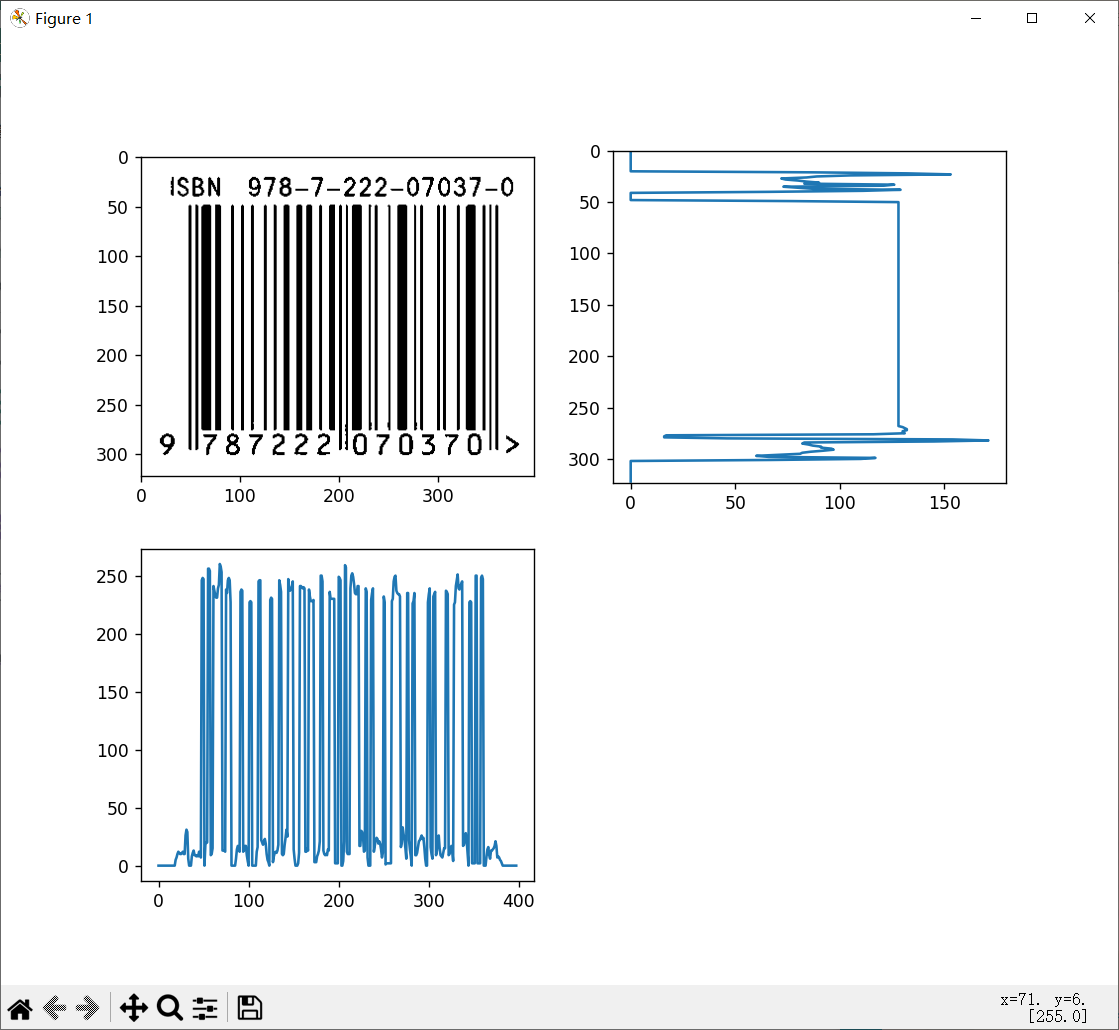
\includegraphics[height=260pt]{isbn_sum}
    \caption{ISBN图的统计特征}
\end{figure}

观察图像可知,垂直统计图的条形码处的波形波动也跟条形码一样剧烈变化,且水平统计图的条形码处是一段平的较高的图形。而ISBN号一定出现在其条形码的上下两端出现。根据ISBN号的知识可知,上下出现的数字一定是相同的。则任取一边进行识别即可。比较显然下方的数字更好处理,所以优先考虑识别下边的数字。

数字区域的水平特征是,出现在条形码区域的附近,且边界是低频率的。那么我们可以先按水平特征截取出数字行,再进一步分析。在实现上,可以设一个低频阈值 $low$,如果某一行出现黑点个数 $\ge low$,就开始记为边界,直到下一次再出现 $< low$ 的行就设为另一边界,并把边界之间的行全部提取出来。根据肉眼观察和经验推理,不妨预设 $low=25\%max$,即最高频次的 $25\%$。

核心代码如下:
\begin{lstlisting}[language=python]
def getNumberLineRange(sumHori, low=0.25):
    lim = np.max(sumHori)*low  # 实际阈值
    left, right = -1, -1
    n = sumHori.shape[0]
    for i in range(n-1, -1, -1):
        if sumHori[i] >= lim and right == -1:
            right = i
        if sumHori[i] < lim and right != -1:
            left = i
            break
    return [max(0, left), max(0, right)]
\end{lstlisting}

分割效果如下:
\begin{figure}[H]
    \centering
    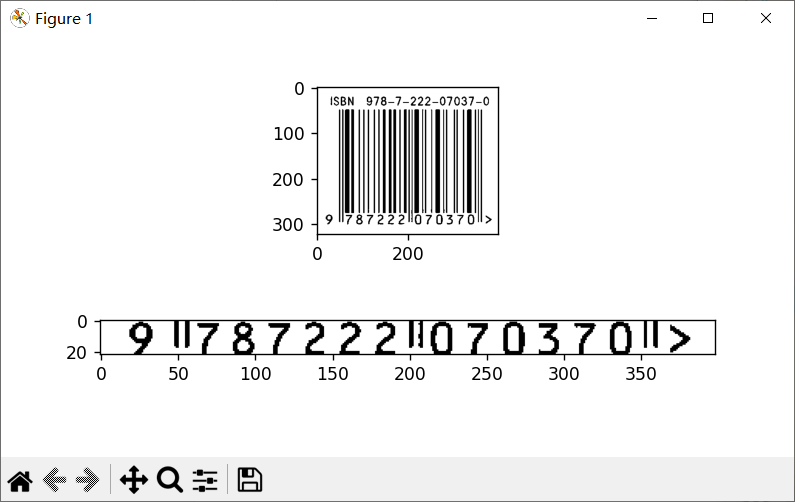
\includegraphics[height=120pt]{sample_splitRow}
    \caption{按行分割效果}
\end{figure}

将其按行分割后,再次求其列特征,调用上述函数,得到统计图如下:
\begin{figure}[H]
    \centering
    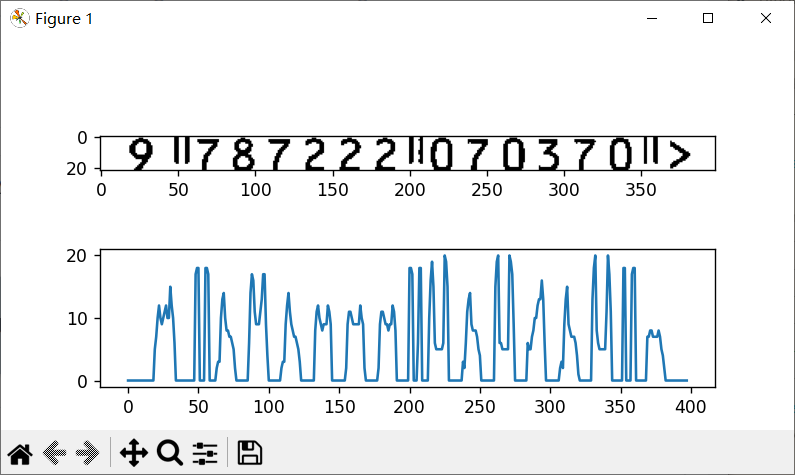
\includegraphics[height=120pt]{sample_splitRow_ana}
    \caption{按行分割后的按行统计图}
\end{figure}

可以发现,每个数字都对应一段连续的波。按照类似上面的办法将其分割即可。直接调整上述代码\textit{(见附录)},得到效果如下:
\begin{figure}[H]
    \centering
    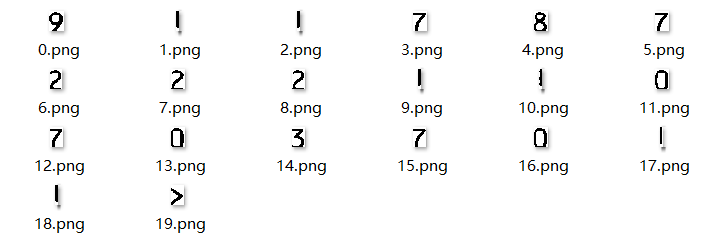
\includegraphics[height=100pt]{sample_splitNum}
    \caption{分割后得到的每个字符}
\end{figure}

可以发现,分割出来的内容里含有无关的元素,包括 ISBN 条形码的多余部分,还有 > 符号。对复杂的图像,可能还有一些噪声、误点等。考虑如何初步筛除这些内容。

关于图像去噪,可以用滤波器等方法先做预处理。对污点
考虑到ISBN里数字都是等大小的,我们可以取截取出来的长度中位数作为判定标准,如果某个区域明显比中位数小,例如不妨设比中位数的 $0.3$ 还要小,就把这个区域给删除掉。注意到在某些字体里,数字 $1$ 可能很小,这样有可能会误删数字 $1$。但是无论如何,条形码横线理论上会比数字 $1$ 更小。且如果是下面截断的 ISBN,条形码最多只有六条。也可以利用这个性质,最多只删除最短的六个区域,能够较大程度确保不会误删(但是有污点时可能少删)。对特殊符号 > 和其他元素的筛除,可能需要进行下一步计算匹配时再处理。

一种实现代码如下:
\begin{lstlisting}[language=python]
def filtRanges(arr, low=0.3, maxDel=6):
    n = len(arr)
    b = [(i, arr[i][1]-arr[i][0]) for i in range(n)]
    b.sort(key=lambda v: v[1])  # 按长度排序
    lim = low*b[n//2][1]  # 中位数
    ban = {b[i][0] for i in range(min(maxDel, n))
           if b[i][1] < lim}
    arr = [arr[i] for i in range(n) if i not in ban]
    return arr
\end{lstlisting}

效果如下,对条形码竖线效果显著:
\begin{figure}[H]
    \centering
    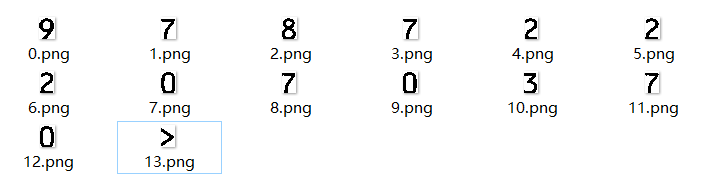
\includegraphics[height=85pt]{sample_splitNum_flit}
    \caption{分割后得到的每个字符(经初步筛查)}
\end{figure}

\subsection{预处理旋转}


\section{实验结果及分析}
\section{总结与体会}
\section{致谢}
\section{参考文献}
Otsu 算法解析\\https://blog.csdn.net/a15779627836/article/details/124151125
\section{附录}
\end{document}